\documentclass[12pt,a4paper]{article}
\usepackage[utf8]{inputenc}
\usepackage[T1]{fontenc}
\usepackage[margin=2.5cm]{geometry}
\usepackage{graphicx}
\usepackage{hyperref}
\usepackage{enumitem}
\usepackage{xcolor}
\usepackage{fancyhdr}
\usepackage{titlesec}
\usepackage{listings}

\definecolor{primary}{RGB}{220, 38, 38}
\definecolor{codebg}{RGB}{248, 249, 250}
\definecolor{pass}{RGB}{34, 197, 94}
\definecolor{fail}{RGB}{239, 68, 68}

\lstset{
    backgroundcolor=\color{codebg},
    basicstyle=\ttfamily\small,
    breaklines=true,
    frame=single,
    language=JavaScript
}

\hypersetup{
    colorlinks=true,
    linkcolor=primary,
    urlcolor=primary
}

\pagestyle{fancy}
\fancyhf{}
\fancyhead[L]{Software Development Project}
\fancyhead[R]{Lecture 9: Testing \& QA}
\fancyfoot[C]{\thepage}

\title{\textbf{Lecture 9: Testing and Quality Assurance}\\[0.5cm]\large Ensuring Your Software Works Correctly}
\author{State University of Zanzibar (SUZA)\\BSc Computer Science}
\date{}

\begin{document}

\maketitle
\tableofcontents
\newpage

\section{Introduction to Software Testing}

\subsection{What is Software Testing?}
Software testing is the process of evaluating software to find defects and verify that it meets specified requirements.

\subsection{Why Testing Matters}
\begin{itemize}
    \item \textbf{Cost:} Finding bugs early is 100x cheaper than fixing them in production
    \item \textbf{Quality:} Ensures software meets user expectations
    \item \textbf{Reliability:} Builds confidence in the software
    \item \textbf{Security:} Identifies vulnerabilities before deployment
    \item \textbf{Documentation:} Tests serve as living documentation
\end{itemize}

\subsection{Testing Pyramid}

\begin{center}
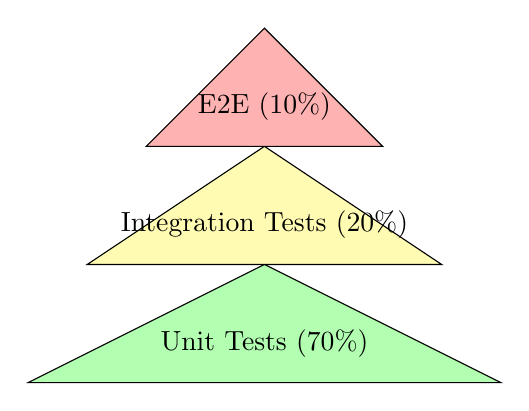
\begin{tikzpicture}
    \draw[fill=green!30] (0,0) -- (6,0) -- (3,1.5) -- cycle;
    \draw[fill=yellow!30] (0.75,1.5) -- (5.25,1.5) -- (3,3) -- cycle;
    \draw[fill=red!30] (1.5,3) -- (4.5,3) -- (3,4.5) -- cycle;

    \node at (3,0.5) {Unit Tests (70\%)};
    \node at (3,2) {Integration Tests (20\%)};
    \node at (3,3.5) {E2E (10\%)};
\end{tikzpicture}
\end{center}

\section{Types of Testing}

\subsection{Unit Testing}

\textbf{What:} Testing individual functions or components in isolation.

\textbf{Characteristics:}
\begin{itemize}
    \item Tests smallest testable parts
    \item Fast execution
    \item Should be automated
    \item Run frequently (on every commit)
\end{itemize}

\textbf{Example (JavaScript with Jest):}
\begin{lstlisting}
// Function to test
function add(a, b) {
    return a + b;
}

// Unit test
describe('add function', () => {
    test('adds two positive numbers', () => {
        expect(add(2, 3)).toBe(5);
    });

    test('adds negative numbers', () => {
        expect(add(-1, -1)).toBe(-2);
    });

    test('adds zero', () => {
        expect(add(5, 0)).toBe(5);
    });
});
\end{lstlisting}

\textbf{Example (Python with pytest):}
\begin{lstlisting}[language=Python]
# Function to test
def calculate_discount(price, discount_percent):
    if discount_percent < 0 or discount_percent > 100:
        raise ValueError("Invalid discount")
    return price * (1 - discount_percent / 100)

# Unit tests
def test_calculate_discount_normal():
    assert calculate_discount(100, 20) == 80

def test_calculate_discount_zero():
    assert calculate_discount(100, 0) == 100

def test_calculate_discount_invalid():
    with pytest.raises(ValueError):
        calculate_discount(100, 150)
\end{lstlisting}

\subsection{Integration Testing}

\textbf{What:} Testing how components work together.

\textbf{Examples:}
\begin{itemize}
    \item API endpoint tests
    \item Database operations
    \item External service integrations
\end{itemize}

\textbf{Example (API Test):}
\begin{lstlisting}
describe('User API', () => {
    test('POST /users creates new user', async () => {
        const response = await request(app)
            .post('/api/users')
            .send({
                name: 'John Doe',
                email: 'john@example.com',
                password: 'password123'
            });

        expect(response.status).toBe(201);
        expect(response.body.data.name).toBe('John Doe');
    });

    test('GET /users/:id returns user', async () => {
        const response = await request(app)
            .get('/api/users/1');

        expect(response.status).toBe(200);
        expect(response.body.data.id).toBe(1);
    });
});
\end{lstlisting}

\subsection{End-to-End (E2E) Testing}

\textbf{What:} Testing complete user workflows.

\textbf{Tools:} Cypress, Selenium, Playwright

\textbf{Example (Cypress):}
\begin{lstlisting}
describe('User Login', () => {
    it('should login successfully', () => {
        cy.visit('/login');
        cy.get('input[name="email"]').type('user@example.com');
        cy.get('input[name="password"]').type('password123');
        cy.get('button[type="submit"]').click();
        cy.url().should('include', '/dashboard');
        cy.contains('Welcome').should('be.visible');
    });

    it('should show error for invalid credentials', () => {
        cy.visit('/login');
        cy.get('input[name="email"]').type('wrong@example.com');
        cy.get('input[name="password"]').type('wrongpassword');
        cy.get('button[type="submit"]').click();
        cy.contains('Invalid credentials').should('be.visible');
    });
});
\end{lstlisting}

\subsection{Other Testing Types}

\begin{tabular}{|l|p{8cm}|}
\hline
\textbf{Type} & \textbf{Purpose} \\
\hline
Smoke Testing & Quick test to ensure basic functionality works \\
\hline
Regression Testing & Verify changes don't break existing features \\
\hline
Performance Testing & Test speed, scalability, stability \\
\hline
Security Testing & Find vulnerabilities \\
\hline
Usability Testing & Evaluate user experience \\
\hline
UAT & User validates requirements are met \\
\hline
\end{tabular}

\section{Test-Driven Development (TDD)}

\subsection{What is TDD?}
Write tests BEFORE writing the code.

\subsection{TDD Cycle: Red-Green-Refactor}

\begin{enumerate}
    \item \textcolor{fail}{\textbf{RED:}} Write a failing test
    \item \textcolor{pass}{\textbf{GREEN:}} Write minimal code to pass the test
    \item \textbf{REFACTOR:} Improve code while keeping tests green
\end{enumerate}

\subsection{TDD Example}

\textbf{Step 1: Write failing test (RED)}
\begin{lstlisting}
test('should validate email format', () => {
    expect(isValidEmail('test@example.com')).toBe(true);
    expect(isValidEmail('invalid-email')).toBe(false);
});
// Test fails - function doesn't exist yet!
\end{lstlisting}

\textbf{Step 2: Write minimal code (GREEN)}
\begin{lstlisting}
function isValidEmail(email) {
    const regex = /^[^\s@]+@[^\s@]+\.[^\s@]+$/;
    return regex.test(email);
}
// Test passes!
\end{lstlisting}

\textbf{Step 3: Refactor if needed}
\begin{lstlisting}
// Add more robust validation if needed
function isValidEmail(email) {
    if (!email || typeof email !== 'string') return false;
    const regex = /^[^\s@]+@[^\s@]+\.[^\s@]+$/;
    return regex.test(email.trim());
}
\end{lstlisting}

\section{Writing Good Test Cases}

\subsection{Test Case Structure: AAA Pattern}

\begin{itemize}
    \item \textbf{Arrange:} Set up test data and conditions
    \item \textbf{Act:} Execute the function/action being tested
    \item \textbf{Assert:} Verify the expected outcome
\end{itemize}

\begin{lstlisting}
test('should calculate total with discount', () => {
    // Arrange
    const cart = {
        items: [
            { price: 100, quantity: 2 },
            { price: 50, quantity: 1 }
        ],
        discountPercent: 10
    };

    // Act
    const total = calculateTotal(cart);

    // Assert
    expect(total).toBe(225); // (200 + 50) * 0.9
});
\end{lstlisting}

\subsection{Test Case Template}

\begin{tabular}{|l|p{8cm}|}
\hline
\textbf{Test Case ID} & TC-001 \\
\hline
\textbf{Title} & User can login with valid credentials \\
\hline
\textbf{Preconditions} & User account exists in database \\
\hline
\textbf{Test Steps} &
1. Navigate to login page\\
2. Enter valid email\\
3. Enter valid password\\
4. Click login button \\
\hline
\textbf{Expected Result} & User is redirected to dashboard \\
\hline
\textbf{Actual Result} & [Fill during execution] \\
\hline
\textbf{Status} & Pass / Fail \\
\hline
\end{tabular}

\subsection{What to Test}

\begin{itemize}
    \item \textbf{Happy path:} Normal, expected usage
    \item \textbf{Edge cases:} Boundary values, empty inputs
    \item \textbf{Error cases:} Invalid input, exceptions
    \item \textbf{Security:} Authentication, authorization
\end{itemize}

\section{Testing Tools}

\subsection{JavaScript/Node.js}

\begin{tabular}{|l|l|}
\hline
\textbf{Tool} & \textbf{Purpose} \\
\hline
Jest & Unit testing, mocking \\
\hline
Mocha + Chai & Flexible testing framework \\
\hline
Supertest & API testing \\
\hline
Cypress & E2E testing \\
\hline
\end{tabular}

\subsection{Python}

\begin{tabular}{|l|l|}
\hline
\textbf{Tool} & \textbf{Purpose} \\
\hline
pytest & Unit testing \\
\hline
unittest & Built-in testing \\
\hline
Selenium & Browser automation \\
\hline
\end{tabular}

\subsection{Java}

\begin{tabular}{|l|l|}
\hline
\textbf{Tool} & \textbf{Purpose} \\
\hline
JUnit & Unit testing \\
\hline
Mockito & Mocking \\
\hline
Selenium & Browser automation \\
\hline
\end{tabular}

\section{Bug Reporting}

\subsection{Bug Report Template}

\begin{tabular}{|l|p{8cm}|}
\hline
\textbf{Bug ID} & BUG-001 \\
\hline
\textbf{Title} & Login fails with special characters in password \\
\hline
\textbf{Severity} & High \\
\hline
\textbf{Environment} & Chrome 120, Windows 11 \\
\hline
\textbf{Steps to Reproduce} &
1. Go to login page\\
2. Enter email: test@example.com\\
3. Enter password: P@ss\#word!\\
4. Click login \\
\hline
\textbf{Expected} & User logs in successfully \\
\hline
\textbf{Actual} & Error: "Invalid characters" \\
\hline
\textbf{Screenshot} & [Attach image] \\
\hline
\end{tabular}

\subsection{Bug Severity Levels}

\begin{itemize}
    \item \textbf{Critical:} System crash, data loss, security breach
    \item \textbf{High:} Major feature broken, no workaround
    \item \textbf{Medium:} Feature partially broken, workaround exists
    \item \textbf{Low:} Minor issue, cosmetic problems
\end{itemize}

\section{Code Coverage}

\subsection{What is Code Coverage?}
Percentage of code executed during testing.

\subsection{Coverage Types}
\begin{itemize}
    \item \textbf{Line coverage:} Lines of code executed
    \item \textbf{Branch coverage:} Decision branches taken
    \item \textbf{Function coverage:} Functions called
\end{itemize}

\subsection{Coverage Goals}
\begin{itemize}
    \item Aim for 80\%+ coverage
    \item 100\% coverage doesn't mean bug-free
    \item Focus on critical paths
\end{itemize}

\textbf{Running coverage (Jest):}
\begin{lstlisting}[language=bash]
npm test -- --coverage
\end{lstlisting}

\section{Continuous Testing}

\subsection{CI/CD Integration}

Run tests automatically on:
\begin{itemize}
    \item Every commit
    \item Pull requests
    \item Before deployment
\end{itemize}

\textbf{GitHub Actions Example:}
\begin{lstlisting}
name: Tests
on: [push, pull_request]
jobs:
  test:
    runs-on: ubuntu-latest
    steps:
      - uses: actions/checkout@v3
      - uses: actions/setup-node@v3
      - run: npm install
      - run: npm test
\end{lstlisting}

\section{Practical Exercise}

For your project, implement:

\begin{enumerate}
    \item At least 10 unit tests for core functions
    \item At least 3 integration tests for API endpoints
    \item Test coverage report
    \item Bug report for any issues found
\end{enumerate}

\section{Summary}

\begin{itemize}
    \item Testing is essential for quality software
    \item Follow the testing pyramid: many unit tests, fewer E2E tests
    \item Use TDD to write better code
    \item Automate tests in CI/CD pipeline
    \item Document bugs clearly with steps to reproduce
    \item Aim for meaningful coverage, not just numbers
\end{itemize}

\end{document}
